\documentclass[a0,portrait]{a0poster}

\usepackage{multicol}
\usepackage{multirow}

\columnsep=100pt
\columnseprule=3pt
\usepackage[svgnames]{xcolor} 
\usepackage{times}
\usepackage{palatino}
\usepackage{graphicx}
\graphicspath{{figures/}}
\usepackage{booktabs}
\usepackage[font=small,labelfont=bf]{caption}
\usepackage{amsfonts, amsmath, amsthm, amssymb}
\usepackage{wrapfig}
\usepackage{url}
\usepackage{color}

\usepackage{minted}
\usemintedstyle{vs}
\begin{document}

\begin{minipage}[b]{0.75\linewidth}
\VeryHuge \color{NavyBlue}\textbf{AriaDB: A key-value store in Haskell}\color{Black}\\[2.0cm]
\huge \textbf{Abhilash Kumar, Proneet Verma and Saurav Kumar}\\[0.8cm]
\huge Indian Institute of Technology Kanpur \\[0.4cm] 
\Large \texttt{\{abhilak, proneetv, ksaurav\} @iitk.ac.in}\\
\end{minipage}
% 
\begin{minipage}[b]{0.25\linewidth}

\includegraphics[width=7cm]{iitk.png}\ 

\includegraphics[width=10cm]{haskell.png}\\
\end{minipage}
\vspace{1cm} % A bit of extra whitespace between the header and poster content

%----------------------------------------------------------------------------------------

\begin{multicols}{2} % This is how many columns your poster will be broken into, a portrait poster is generally split into 2 columns

% Things to put:
%  1. Abstract
%  2. Introduction
%  3. Motivation
%  4. Design (BPT, Warp, Library)
%  5. Features (BPT index, loose coupling b/w service and lib: spring like, inherent concurrency, ..., ?Caching, )
%  6. Implementation (pseudo codes, documentation)
%  7. Data and Graphs : Read Write speed. Compare with UTree (no-index)
%  8. 

\color{Navy}

\begin{abstract}
Key-value stores are an essential component in the industry, including social networks and online retail. Apart from performance, today we need concise, elegant, concurrent, type-safe and maintainable code. We present \textbf{ariaDB}, a persistent key-value store written in Haskell and a library to use the service in Haskell language. The datastore uses B+ tree to index the data for faster reads and writes. 
\end{abstract}

\color{Black}
\section*{Introduction}
The aim was not to implement another key value store, but to implement a key-value store in Haskell. Infact, this key-value data store is inspired from NoSQL databases which are based on the idea of a B+ Tree indexed structure.

Haskell is a purely functional, statically typed and lazy language. Writing a program in Haskell requires thinking functionally and is quite different from programming in imperative languages like C++/Java.

\color{Black}

\section*{Design}
AriaDB is designed to have an uncoupled service and client utility. AriaDB server has a datastore which is indexed using B+ tree, and it exposes REST APIs to talk to AriaDB clients. In addition to the service, we have also implemented the client library for Haskell language, which can easily be extended over to any number of languages.
\begin{center}\vspace{1cm}
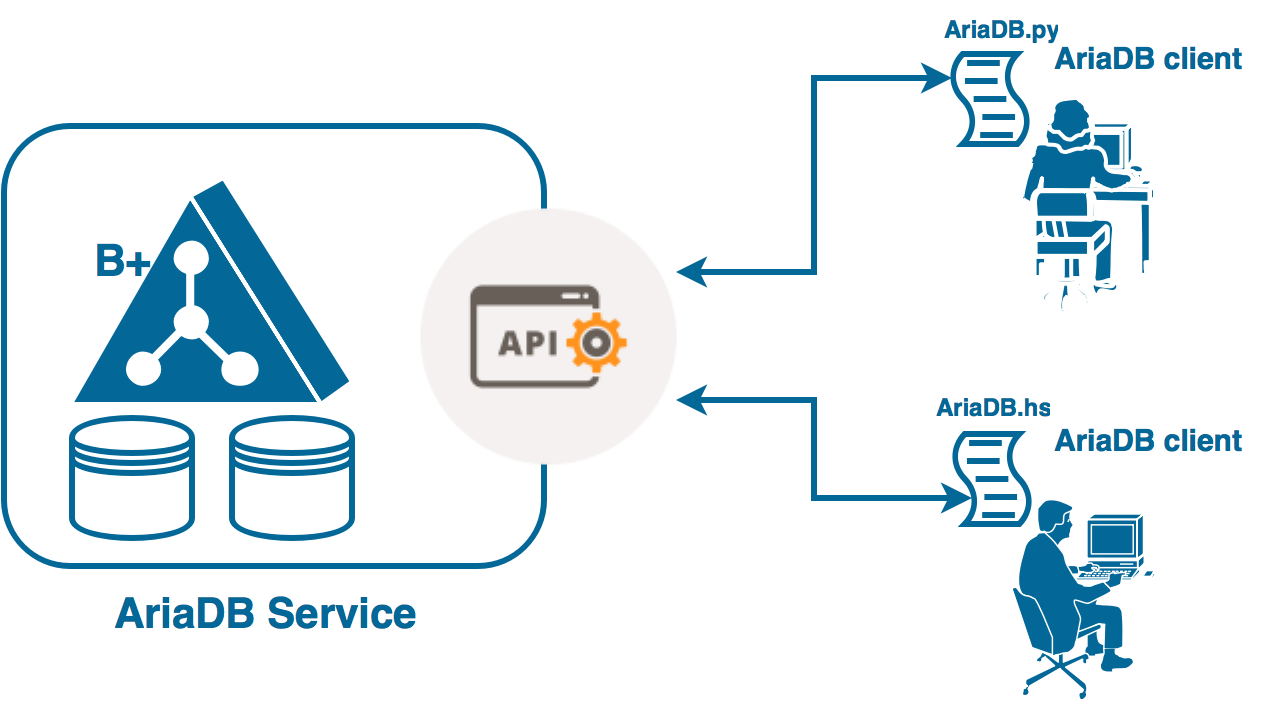
\includegraphics[width=0.8\linewidth]{ariaDB}
\captionof{figure}{\color{Green}Design of AriaDB: separate server module and client libraries}
\end{center}

\subsection*{Server}
This is the HTTP API layer of the database and serves the endpoints to which the clients talk  to exchange data. This is where the requests like GET, PUT and DELETE are handled. Irregular behavior is error-handled here itself.

\subsection*{B+ Tree}
B+ Trees are primarily used here to keep data indexed based on their keys, thereby enhancing the retrieval of data. Its a disk based index structure which in turn powers up our datastore to be persistent, since in-memory structures have size restrictions. 

\subsection*{Caching}
Since our index structure is a disk based one, concurrent disk IO is one of the biggest hindrance to the performance of our database. Hence, we have implemented a in-memory caching layer to avoid repeated disk IOs and thereby improving read speed by a substantial factor.

\subsection*{Client}
This is the interface to ariaDB server with which the user interacts with the datastore. This module basically packs the HTTP Request and sends to the server. Hence, the way our database interaction is implemented, clients may interact with the database using any programming language having an HTTP module.\\
\\
The heart of the datastore is in Haskell utilizing all possible functional programming style, and powering the data with concurrent access, faster retrieval and caching but the user can interact with it using any style of programming with the only requirement that it must have an HTTP module.

\section*{Features \& their implementation}
\begin{description}
  \item[Indexing:] \hfill \\
  Implemented a B+ Tree index structure to index the \textbf{AriaValue} based on the \textbf{AriaKey}.
  \item[Uncoupled Service and Library:] \hfill \\
  Using the Haskell \textbf{Warp} module, we have implemented REST APIs which responds to clients HTTP requests and thereby serving the interface layer between the client and the datastore.
  \item[Caching:] \hfill \\
  This layer is based on a \textbf{Least-Recently-Used Caching} model. Least frequently queried keys are highly likely to be removed from the in-memory store and replaced by newer keys. 
\end{description}

\subsection*{Pseudo Code}
\begin{minipage}[b]{0.5\linewidth}
\begin{minted}{haskell}
-- Types
type AriaKey    = String
type AriaValue  = String
data AriaKV = AriaKV {
  key :: AriaKey,
  value :: AriaValue
 } deriving (Show, Read)

-- Client Library
get :: (Read a) => AriaKey 
	-> IO (Maybe a)
put :: (Show a) => AriaKey -> a
	-> IO ()
delete :: AriaKey -> IO ()

-- Request Handling at Warp Server
app req respond =
case requestMethod req of
 "GET" -> case pathInfo req of
 [key] -> do
  value <- Cache.get lruCache key
  case value of
   Just v  -> respond200With v
   Nothing -> respond notFound
  _ -> respond forbidden

 "POST" -> case pathInfo req of
  [key] -> do
   value <- requestBody req
   Cache.upsert lruCache key value
   respond200With ""
   _ -> respond forbidden

 "DELETE" -> case pathInfo req of
  [key] -> do
   Cache.remove lruCache key
   respond200With ""
   _ -> respond forbidden
_ -> respond forbidden

\end{minted}
\end{minipage}
\begin{minipage}[b]{0.5\linewidth}
\begin{minted}{haskell}
  -- B Plus Tree
  get :: AriaKey -> IO (Maybe AriaValue)
  upsert :: AriaKV -> IO ()
  remove :: AriaKey -> IO ()

--Cache
get :: IORef (LRU AriaKey AriaValue)
 -> AriaKey -> IO (Maybe AriaValue)
upsert :: IORef (LRU AriaKey AriaValue)
 -> AriaKey -> AriaValue -> IO ()
remove :: IORef (LRU AriaKey AriaValue)
 -> AriaKey -> IO ()
 
  -- Usage
  import AriaDB
  data Person = Person {
    firstName :: String,
    lastName  :: String
  } deriving (Show, Read, Eq)
  
  foo = Person "John" "Doe"
  main = do
    let testKey = "k1"
    put testKey foo
    
    bar <- get testKey
    case bar of   -- Type Assigned
        Just v  -> print (v::Person)
        Nothing -> print "Nothing"
        
    baz <- get testKey
    case baz of   -- Type Inferred
      Just v -> print $ v == foo
      Nothing -> print "Not found"
      
    delete testKey
    qux <- get testKey
    case qux of    -- Type Assigned
      Just v  -> print (v::Person)
      Nothing -> print "Nothing"
\end{minted}
\end{minipage}

\section*{Analysis}
\begin{center}
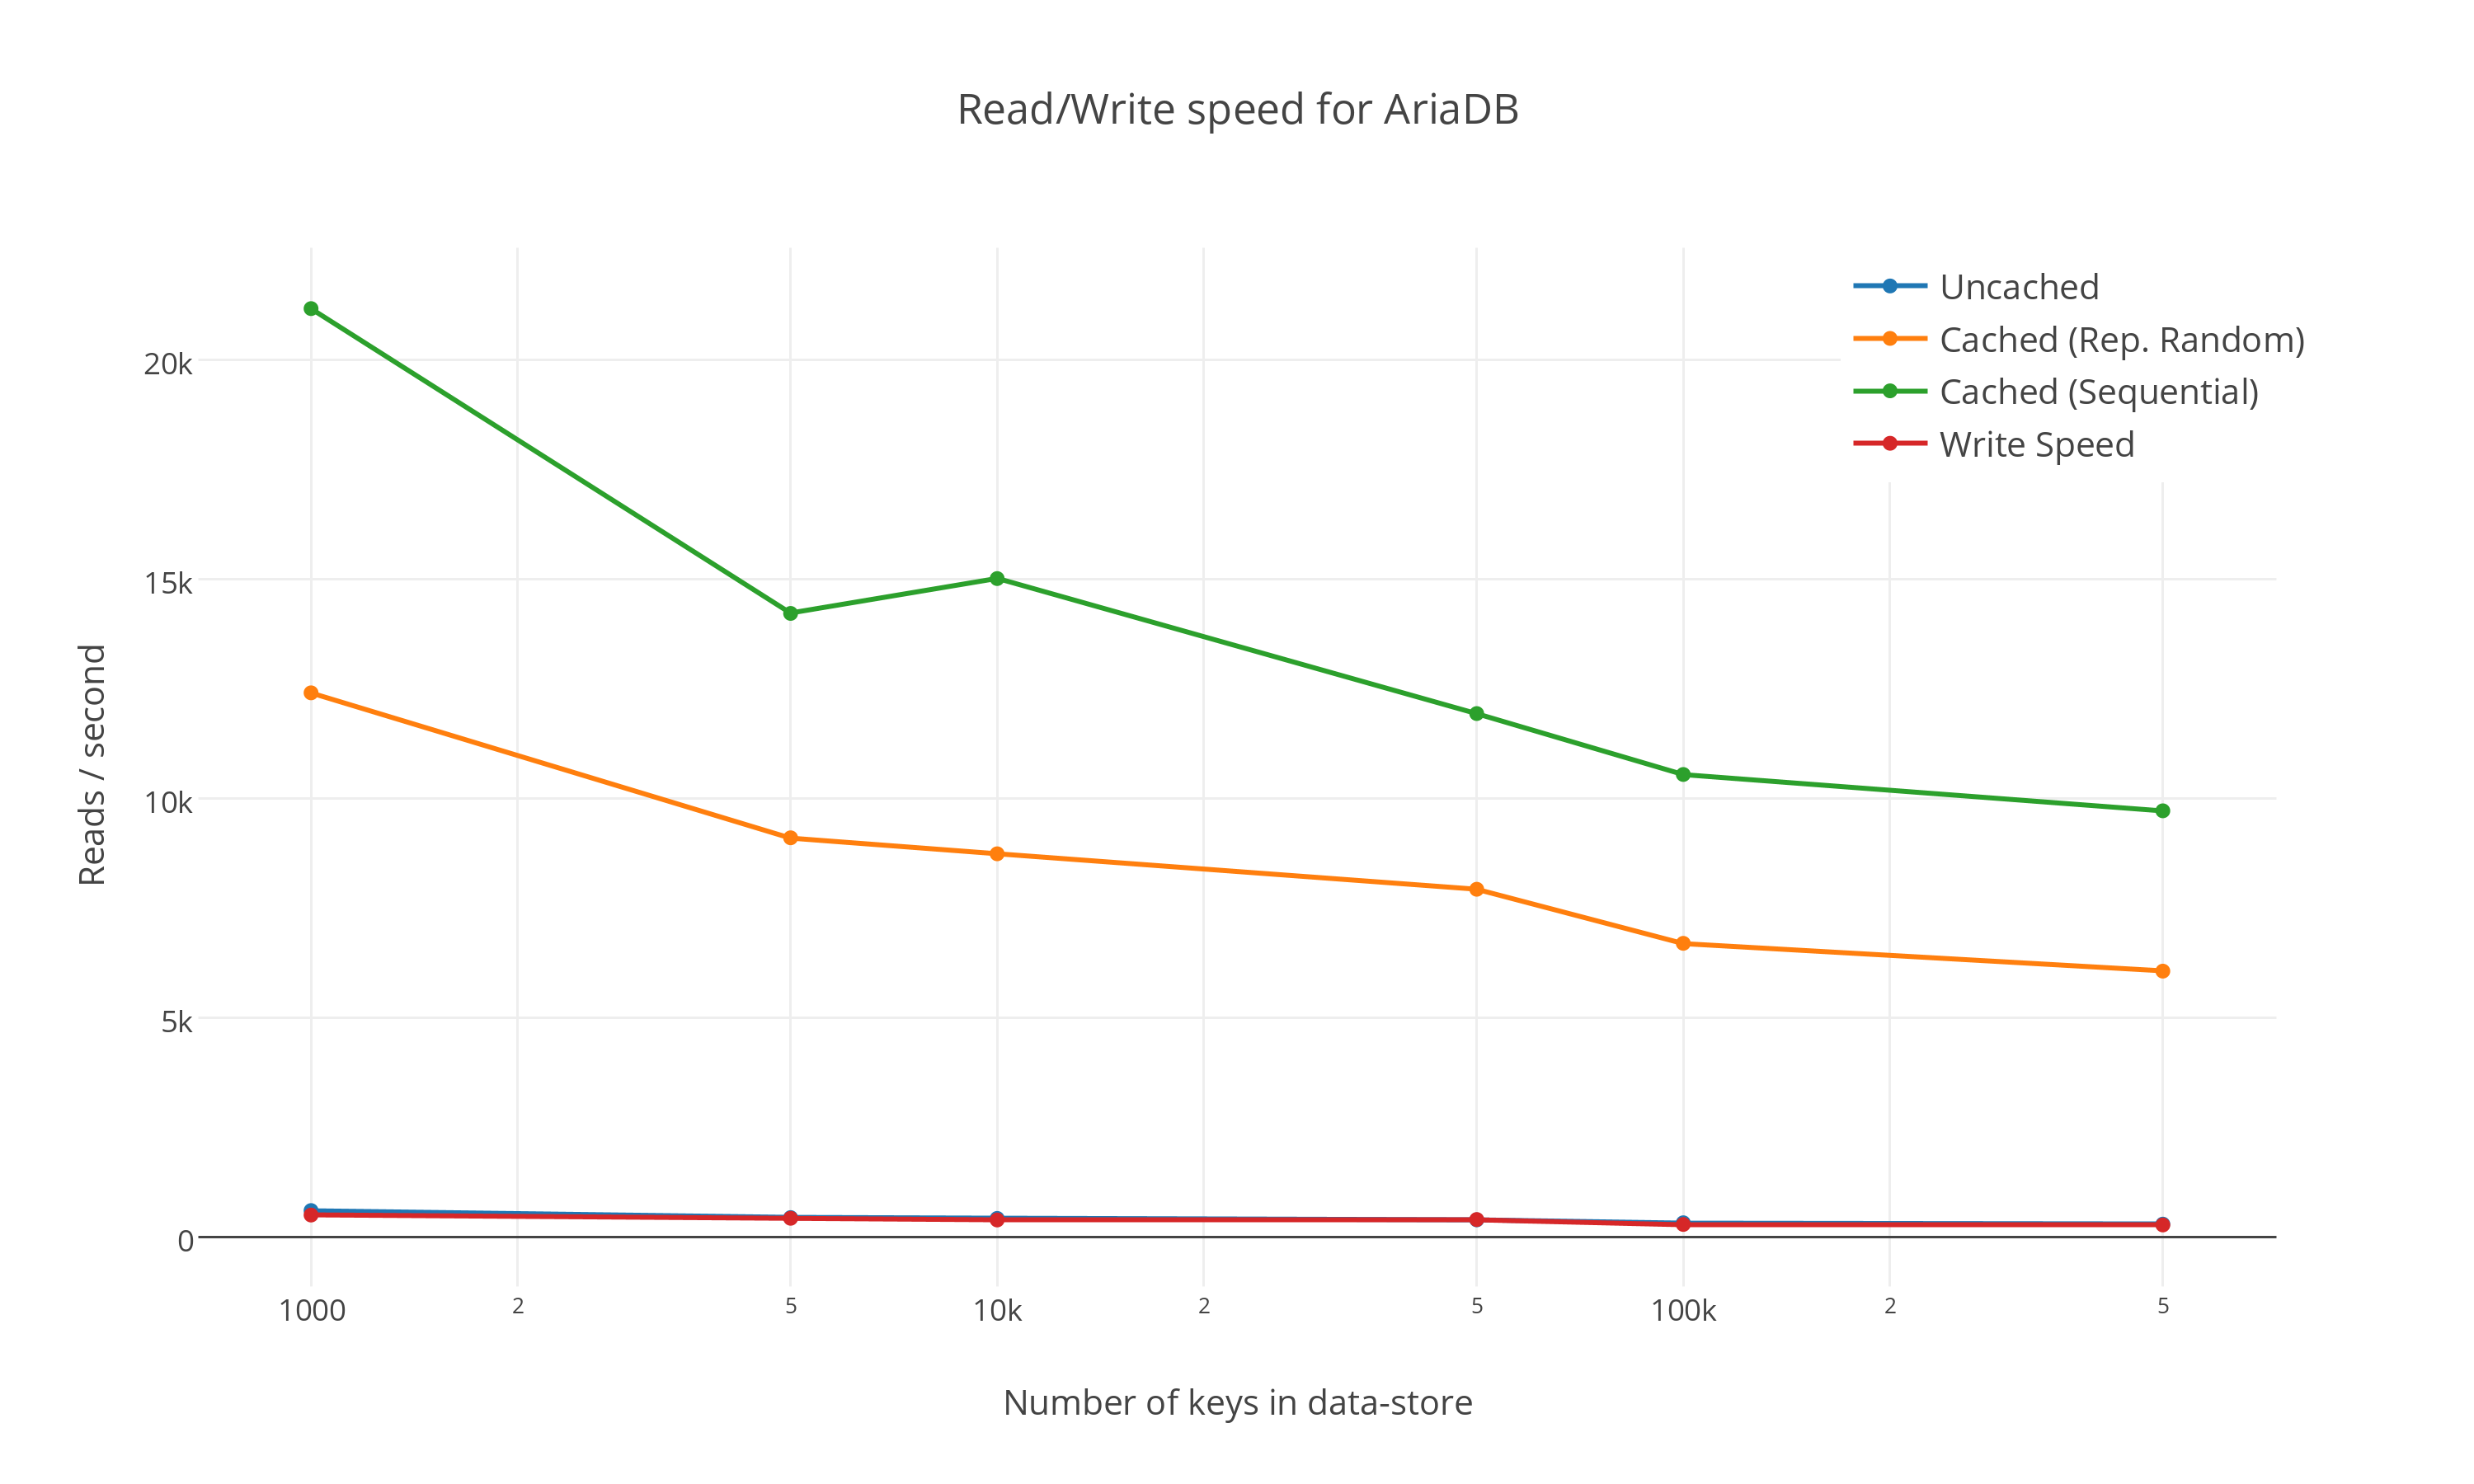
\includegraphics[width=1.0\linewidth]{rw}
\captionof{figure}{\color{Green}Read Write speed vs number of keys in the data store}
\end{center}
\section*{Future Works}
\begin{description}
  \item[R/W Buffers:] As of now, disk IOs happen each time the user tries inserting values, and since disk reads are time consuming; decreasing this disk IO with the help of flushing the buffer to disk would make the design more time efficient.  
  \item[Compaction:] After deletion of key-value pairs, there are much wasted space in the index tree, so re-indexing after a period of time will make this more space efficient.
  \item[Distributed Store:] Currently the database server assumes the datastore to reside on the same machine. But in future, since the data might scale to humongous size, implementing a store in a multinode environment efficiently would help ariaDB in scaling well.
\end{description}
\nocite{*}
\bibliographystyle{plain}
\bibliography{sample}

%----------------------------------------------------------------------------------------

\end{multicols}
\end{document}
